% =====================================================================
% F.CSM302 Үйлдлийн систем - Бие даалт 1
% II-4-6 Multithreaded Sorting Application - Тайлан
%
% Хөрвүүлэх (XeLaTeX шаардлагатай):
%   cd report
%   xelatex main.tex
%   xelatex main.tex        (агуулга, лавлагааг шинэчлэхийн тулд 2 дахь удаа)
% Overleaf: бүх repository-г (src/, docs/images/, tests/results/ хамт) upload хийж,
%   Menu -> Compiler -> XeLaTeX, Main document -> report/main.tex гэж тохируулна.
%
% Зураг: images/ хавтас эсвэл ../docs/images/ хавтсаас хайна. Файл олдохгүй бол
% \shot{...} нь хүрээтэй "энд зураг оруулна" гэсэн хоосон зай зурна.
% =====================================================================
\documentclass[12pt,a4paper,oneside]{report}

% ---------------------------------------------------------------- fonts & language
\usepackage{fontspec}
\usepackage{polyglossia}
\setdefaultlanguage{russian}   % Cyrillic hyphenation (polyglossia has no Mongolian module)
\setotherlanguage{english}
\IfFontExistsTF{DejaVu Serif}{
  \def\mainfam{DejaVu Serif}\def\sansfam{DejaVu Sans}\def\monofam{DejaVu Sans Mono}
}{
  \def\mainfam{Times New Roman}\def\sansfam{Arial}
  \IfFontExistsTF{Menlo}{\def\monofam{Menlo}}{\def\monofam{Courier New}}
}
\setmainfont{\mainfam}
\setsansfont{\sansfam}
\setmonofont{\monofam}[Scale=0.84]
\newfontfamily\cyrillicfont{\mainfam}
\newfontfamily\cyrillicfontsf{\sansfam}
\newfontfamily\cyrillicfonttt{\monofam}[Scale=0.84]

% Mongolian names for the automatic headings
\gappto\captionsrussian{%
  \renewcommand{\contentsname}{Агуулга}%
  \renewcommand{\listfigurename}{Зургийн жагсаалт}%
  \renewcommand{\listtablename}{Хүснэгтийн жагсаалт}%
  \renewcommand{\figurename}{Зураг}%
  \renewcommand{\tablename}{Хүснэгт}%
  \renewcommand{\chaptername}{Бүлэг}%
  \renewcommand{\appendixname}{Хавсралт}%
  \renewcommand{\bibname}{Ашигласан материал}%
  \renewcommand{\abstractname}{Хураангуй}}

% ---------------------------------------------------------------- packages
\usepackage[a4paper,left=3cm,right=2cm,top=2.5cm,bottom=2.5cm]{geometry}
\usepackage{setspace}
\setstretch{1.15}
\usepackage{graphicx}
\graphicspath{{images/}{../docs/images/}}
\usepackage{xcolor}
\usepackage{booktabs}
\usepackage{longtable}
\usepackage{tabularx}
\usepackage{array}
\usepackage{multirow}
\usepackage{enumitem}
\usepackage{amsmath}
\usepackage{float}
\usepackage{caption}
\usepackage{subcaption}
\usepackage{titlesec}
\usepackage{fancyhdr}
\usepackage{etoolbox}
\usepackage{listings}
\usepackage{tikz}
\usetikzlibrary{arrows.meta,positioning,calc,fit,shapes.geometric,decorations.pathreplacing,matrix}
\usepackage{pgfplots}
\usepackage{pgfplotstable}
\pgfplotsset{compat=1.17}
\usepackage{tocloft}
\setlength{\cftchapnumwidth}{2.0em}
\setlength{\cftsecnumwidth}{2.6em}
\setlength{\cftsubsecnumwidth}{3.4em}
\renewcommand{\cftchapdotsep}{\cftdotsep}
\usepackage[hidelinks]{hyperref}

\setlist{itemsep=2pt,topsep=4pt}
\emergencystretch=5em
\renewcommand{\arraystretch}{1.25}
\captionsetup{font=small,labelsep=period}
\newcolumntype{Y}{>{\raggedright\arraybackslash}X}

% chapter heading: "1. Удиртгал"
\titleformat{\chapter}[hang]{\normalfont\Large\bfseries\raggedright}{\thechapter.}{0.6em}{}

% Chapters continue on the same page (no page break before each chapter), like the other team reports
\makeatletter
\patchcmd{\chapter}{\if@openright\cleardoublepage\else\clearpage\fi}{\par\vspace{1.2em}}{}{}
\makeatother
\titlespacing*{\chapter}{0pt}{6pt}{10pt}


\setlength{\headheight}{15pt}
\pagestyle{fancy}
\fancyhf{}
\fancyhead[L]{\small II-4-6 Multithreaded Sorting Application}
\fancyhead[R]{\small\nouppercase{\leftmark}}
\fancyfoot[C]{\thepage}
\renewcommand{\headrulewidth}{0.4pt}
\fancypagestyle{plain}{\fancyhf{}\fancyfoot[C]{\thepage}\renewcommand{\headrulewidth}{0pt}}

% ---------------------------------------------------------------- colours (same as the web UI)
\definecolor{cleft}{HTML}{2F5BEA}
\definecolor{cright}{HTML}{D9860B}
\definecolor{cmerge}{HTML}{0E9A73}
\definecolor{cparent}{HTML}{6B7385}
\definecolor{ccmp}{HTML}{C2185B}
\definecolor{cink}{HTML}{1B2433}
\definecolor{cused}{HTML}{C9CFD8}
\definecolor{codebg}{HTML}{F5F7F9}

% ---------------------------------------------------------------- code listings
\lstdefinestyle{java}{
  language=Java,
  basicstyle=\ttfamily\footnotesize,
  keywordstyle=\color{cleft}\bfseries,
  commentstyle=\color{cparent}\itshape,
  stringstyle=\color{cmerge},
  backgroundcolor=\color{codebg},
  frame=single, rulecolor=\color{cused},
  numbers=left, numberstyle=\tiny\color{cparent}, numbersep=6pt,
  xleftmargin=1.6em, framexleftmargin=1.4em,
  breaklines=true, showstringspaces=false, tabsize=4,
  extendedchars=true, inputencoding=utf8,
  captionpos=b
}
\lstdefinestyle{shell}{
  basicstyle=\ttfamily\footnotesize, backgroundcolor=\color{codebg},
  frame=single, rulecolor=\color{cused}, breaklines=true, columns=fullflexible,
  extendedchars=true
}
\lstset{style=java}
\renewcommand{\lstlistingname}{Код}
\renewcommand{\lstlistlistingname}{Кодын жагсаалт}

% ---------------------------------------------------------------- helpers
\newcommand{\code}[1]{\texttt{#1}}
% \shot{file}{caption}{label}: real screenshot if the file exists, otherwise a framed placeholder
\newcommand{\shot}[3]{%
  \begin{figure}[htbp]\centering
  \IfFileExists{images/#1}{\includegraphics[width=0.82\linewidth]{#1}}{%
  \IfFileExists{../docs/images/#1}{\includegraphics[width=0.82\linewidth]{#1}}{%
    \fbox{\parbox[c][5.5cm][c]{0.9\linewidth}{\centering\color{cparent}
      Энд зураг оруулна:\\[4pt]\texttt{report/images/#1}}}}}
  \caption{#2}\label{#3}
  \end{figure}}

% pgfplots: keep only the rows whose column #1 equals #2 (used for benchmark.csv)
\pgfplotsset{
  only/.style 2 args={
    x filter/.append code={
      \edef\tempa{\thisrow{#1}}\edef\tempb{#2}%
      \ifx\tempa\tempb\else\def\pgfmathresult{inf}\fi}}}
\newcommand{\benchcsv}{../tests/results/benchmark.csv}

% ---------------------------------------------------------------- document data (засах шаардлагатай бол энд)
\newcommand{\University}{ШИНЖЛЭХ УХААН ТЕХНОЛОГИЙН ИХ СУРГУУЛЬ}
\newcommand{\School}{МЭДЭЭЛЭЛ, ХОЛБООНЫ ТЕХНОЛОГИЙН СУРГУУЛЬ}
\newcommand{\Course}{F.CSM302 Үйлдлийн систем}
\newcommand{\Teacher}{Г. Ганбат /F.CS10/}
\newcommand{\RepoURL}{https://github.com/Munkhgerelt/F.CSM302-TeamProject-2-4-6}

\begin{document}

% !TEX root = ../main.tex
% ---------------------------------------------------------------- нүүр хуудас
% Лого: report/images/logo.png. Файл байхгүй бол хүрээтэй хоосон зай гарна.
\begin{titlepage}
    \centering
    \onehalfspacing

    {\large \bfseries \University} \\[0.5cm]
    {\large \School} \\[2cm]

    \IfFileExists{images/logo.png}{%
        
\includegraphics[width=5cm]{images/logo.png}%
    }{%
        \fbox{\parbox[c][4cm][c]{8cm}{\centering\color{cparent} Лого:\\ \texttt{report/images/logo.png}}}%
    } \\[1cm]

    {\Large \bfseries БИЕ ДААЛТ 1} \\[0.3cm]
    {\Large \bfseries ТАЙЛАН} \\[0.5cm]
    {\large \bfseries Үйлдлийн систем (F.CSM302)} \\[2.0cm]

    \begin{raggedleft}
        \begin{tabular}{ll}
            \textbf{Сэдэв:} & Multithreaded Sorting Application, \\
            & Sorting animation \\[0.4cm]
            \textbf{Хуваарилалтын код:} & II-4-6 \\[0.4cm]
            \textbf{Хичээл заасан багш:} & \Teacher \\[0.4cm]
            \textbf{Гүйцэтгэсэн оюутнууд:} & Б. Отгондалай /B241940132/ \\
            & М. Мөнхгэрэлт /B232270012/ \\
            & А. Базарсад /B242270065/ \\
            & Б. Хаш-Эрдэнэ /B241930006/ \\
            & Э. Мичидмаа /B221960015/ \\
            & Ж. Суварнабазар /B251940118/ \\
        \end{tabular}
    \end{raggedleft}

    \vfill

    {\large Улаанбаатар хот, 2026}

\end{titlepage}

\pagenumbering{roman}
% !TEX root = ../main.tex
% ---------------------------------------------------------------- хураангуй
\chapter*{Хураангуй}
\addcontentsline{toc}{chapter}{Хураангуй}

\textbf{Асуудал.} Олон цөмтэй компьютерыг ашиглахын тулд ажлыг thread-үүдэд хуваах шаардлагатай.
Гэхдээ хуваасан ажлын хэсгүүд хэн ямар өгөгдөлд бичих, хэзээ дуусахыг хэрхэн хүлээх, үр дүнг хэрхэн
нэгтгэхийг зөв зохицуулахгүй бол үр дүн буруу гарна. \emph{Operating System Concepts} (10-р хэвлэл) номын
4-р бүлгийн “Multithreaded Sorting Application” төсөл энэ асуудлыг эрэмбэлэлтийн жишээн дээр судалдаг.

\textbf{Шийдэл.} Java 17 дээр жагсаалтыг хоёр хуваан, хоёр \emph{sorting thread} тус бүр параметрээр өгсөн
мужаа эрэмбэлж, гурав дахь \emph{merging thread} эх массивтай ижил хэмжээтэй хоёр дахь global массив руу
нэгтгэдэг програм хийв. Parent thread бүх thread-ийг \code{join()} хийсний дараа үр дүнг хэвлэнэ. Синхрончлолыг
бүхэлд нь \code{start()}/\code{join()} хангадаг тул lock шаардлагагүй. Таван алгоритм (insertion, bubble,
selection, merge, quick), оролтын шалгалт, JSON event trace хийсэн. Мөн бодит thread-тэй холбогдсон хөтчийн
\emph{Sorting animation} хийсэн бөгөөд хоёр горимтой: бүртгэсэн алхмыг тоглуулах \emph{Replay}, амьд thread-ийг
\code{Semaphore}-оор нэг үйлдлээр урагшлуулах \emph{Lockstep}.

\textbf{Туршилт.} JUnit-гүй 100 автомат тест бичиж, macOS (Temurin 17) ба Linux (OpenJDK 21) орчинд ажиллуулав.
Тест нь номын жишээ, захын тохиолдол, буруу оролт, давхардал, $n = 10^6$ хүртэлх том өгөгдөл, thread-ийн
дараалал, trace, Lockstep-ийг хамарна. Хугацааг 1 thread, 1 thread хувааж, 3 thread гэсэн гурван хувилбараар,
3 тусдаа JVM дээр хэмжив.

\textbf{Гол үр дүн.} 100/100 тест амжилттай. Sorter бүр зөвхөн өөрийн мужид бичдэгийг trace-ээс баталсан.
Хоёр цөмтэй машин дээр merge ба quick sort-ын хурдсалт $n = 10^6$ үед $1.7\times$ орчим гарсан. Энэ нь 2-оос
бага бөгөөд шалтгаан нь нэгтгэх үе дан thread-ээр явдагт оршино (Амдалын хууль). O($n^2$) алгоритмд
($n = 20\,000$) insertion ба selection sort-ын хурдсалт $2.4$--$3.6\times$ гарсан ч ашгийн ихэнх нь массивыг
хуваасантай холбоотой, учир нь хоёр хэсгийг эрэмбэлэх ажил $2(n/2)^2 = n^2/2$ байна. $n \le 1000$ үед thread
үүсгэх, \code{join()} хийх зардал давамгайлж, олон урсгалт хувилбар нэг урсгалтаас удаан ажилласан.

\medskip
\noindent\textbf{Түлхүүр үг:} thread, олон урсгалт програмчлал, \code{join}, зэрэгцээ тооцоолол,
эрэмбэлэлт, merge, semaphore, Амдалын хууль, Java.

\tableofcontents
\clearpage
\pagenumbering{arabic}

% !TEX root = ../main.tex
\chapter{Удиртгал}\label{ch:intro}

\section{Зорилго}
\emph{Operating System Concepts} номын 4-р бүлгийн “Multithreaded Sorting Application” төслийг Java 17 дээр
хэрэгжүүлэх нь ажлын зорилго юм. Жагсаалтыг хоёр хуваан хоёр sorting thread-ээр эрэмбэлж, гурав дахь merging
thread-ээр хоёр дахь global массив руу нэгтгэнэ. Thread-ийн бодит ажиллагааг хөтөч дээр \emph{Sorting animation}
хэлбэрээр харуулна. Мөн оролтын шалгалт, автомат тест хийж, олон урсгалт шийдэл хэзээ ашигтай болохыг хугацааны
хэмжилтээр шинжилнэ.

\section{Ач холбогдол}
Орчин үеийн компьютер олон цөмтэй боловч нэг урсгалтай програм тэдгээрийн зөвхөн нэгийг ашигладаг. Ажлыг
thread-үүдэд хуваахад хэн ямар өгөгдөлд бичих, хэзээ дуусахыг хүлээх, үр дүнг хэрхэн нэгтгэх гэсэн асуудал
гарч ирдэг~\cite{osc10}. Энэ төсөл нь \emph{өгөгдлийн зэрэгцээ} (data parallelism) болон \emph{fork--join}
загварыг энгийн жишээн дээр харуулдаг.

\section{Хамрах хүрээ}
Програм нь Java 17-ийн зөвхөн стандарт санг ашиглана. Командын мөр (CLI) болон локал web сервер дээрх хөтчийн
UI гэсэн хоёр интерфейстэй. Утгууд \code{int} мужид байх ба хэмжээний хязгаарыг \ref{sec:limits}-р хэсэгт өгөв.
Эх код, тест, гарын авлага GitHub repository-д байгаа~\cite{repo}.

% !TEX root = ../main.tex
\chapter{Сурах бичгийн шаардлага}\label{ch:req}

\section{Номын үндсэн шаардлага}
Бүхэл тоон жагсаалтыг ижил хэмжээтэй хоёр хэсэгт хувааж, хоёр тусдаа thread тус бүр нэг хэсгийг дурын алгоритмаар
эрэмбэлнэ. Гурав дахь thread хоёр хэсгийг эх массивтай ижил хэмжээтэй хоёр дахь global массив руу нэгтгэнэ.
Parent thread бүх sorting thread дуусахыг хүлээж, дараа нь merging thread-ийг эхлүүлж, түүнийг дуустал хүлээгээд
үр дүнг хэвлэнэ. Thread бүрд эрэмбэлэх хэсгийн эхлэх индекс зэрэг параметрийг дамжуулна~\cite[Ch.~4, Programming Projects]{osc10}.

\section{Нэмэлт шаардлага}
Сэдвийн хуваарилалтаар \emph{Sorting animation} нэмэгдсэн: дүрслэл нь бодит thread-тэй холбоотой байж, хэмжээ ба
утгыг өөрчлөх, Run / Step / Pause / Reset, хурдны удирдлагатай байна. Мөн багшийн заавраар гарын авлага, тайлан,
GitHub repository шаардлагатай. Баг өөрөө оролтын бүрэн шалгалт (хоосон, тоо биш, хэт том утга, $n = 0\dots3$,
давхардал, сондгой $n$) болон зөвхөн стандарт сан ашиглах шаардлагыг тавьсан.

\section{Шаардлагын хангалт}
\begin{table}[H]
\centering\small
\caption{Номын шаардлага ба хэрэгжүүлэлт}\label{tab:req}
\begin{tabularx}{\linewidth}{@{}YY@{}}
\toprule
Шаардлага & Хэрэгжүүлэлт \\
\midrule
Жагсаалтыг хоёр хуваах & \code{splitIndex(n)} $=\lceil n/2\rceil$; зүүн \code{[0, mid)}, баруун \code{[mid, n)} \\
Хоёр sorting thread & \code{SortingThread extends Thread}; 5 алгоритмаас хэсэг тус бүрд сонгоно \\
Global жагсаалт ба хоёр дахь массив & \code{SharedData.list}, \code{SharedData.result = new int[n]} \\
Merging thread & \code{MergingThread}: хоёр заагчтай, тогтвортой нэгтгэл \\
Parent хүлээгээд нэгтгэнэ & \code{left.join(); right.join(); merger.start(); merger.join();} \\
Параметр дамжуулах & \code{SortParams(name, startIndex, endIndex, algorithm)}, \code{MergeParams} \\
Үр дүн хэвлэх & Үр дүн, thread бүрийн статистик, \code{Arrays.sort}-той харьцуулсан шалгалт \\
\bottomrule
\end{tabularx}
\end{table}

\section{Номын жишээ ба сондгой $n$}
Номын жишээ \code{7, 12, 19, 3, 18, 4, 2, 6, 15, 8}-ийн хоёр хэсэг \code{3 7 12 18 19 | 2 4 6 8 15} болж эрэмбэлэгдээд,
\code{2 3 4 6 7 8 12 15 18 19} гэж нэгтгэгдэнэ. Номд хэсгүүдийг “ижил хэмжээтэй” гэсэн ч сондгой $n$ үед энэ
боломжгүй. Бид сондгой $n$-ийг алдаа гэж үзэхийн оронд хэсгүүдийг $\lceil n/2\rceil$ ба $\lfloor n/2\rfloor$ болгосон.
Нэгтгэх алгоритм тэнцүү хэмжээ шаарддаггүй бөгөөд ялгаа нь ердөө 1 элемент юм. $n = 1$ үед баруун хэсэг хоосон
байх ч номын бүтцийг хадгалж Sorter-R thread ажиллаад шууд дуусна.

% !TEX root = ../main.tex
\chapter{Онолын үндэс}\label{ch:theory}

\section{Thread ба зэрэгцээ ажиллагаа}
Thread бол CPU-г ашиглах үндсэн нэгж бөгөөд өөрийн регистр, программ тоолуур, stack-тай. Нэг процессын
thread-үүд code, data хэсэг болон нээлттэй файлаа хуваалцдаг~\cite[4.1]{osc10}. Иймээс манай хоёр sorting thread
ба merging thread нэг процессын хоёр массивт шууд ханддаг. \emph{Concurrency} нь хэд хэдэн ажил зэрэг урагшлахыг,
\emph{parallelism} нь тэдгээр бодитоор өөр өөр цөм дээр нэгэн агшинд гүйцэтгэгдэхийг хэлнэ~\cite[4.2]{osc10}.
Хоёр sorter ижил үйлдлийг өгөгдлийн хоёр хэсэг дээр хийдэг тул энэ нь \emph{өгөгдлийн зэрэгцээ} юм. Parent
thread хүүхэд thread-үүдийг үүсгэж (fork), дуусахыг нь хүлээж (join), дараа нь нэгтгэдэг загварыг
\emph{fork--join} гэнэ~\cite[4.5.2]{osc10}.

\section{Амдалын хууль}
Програмын дараалсан хэсгийн эзлэх хувийг $S$, цөмийн тоог $N$ гэвэл хамгийн их хурдсалт~\cite{amdahl67}
\begin{equation}
  \text{speedup} \le \frac{1}{S + (1-S)/N}.
  \label{eq:amdahl}
\end{equation}
Манай төсөлд нэгтгэх үе дан thread-ээр явдаг тул $S > 0$ бөгөөд $N = 2$ үед ч хурдсалт 2-т хүрэхгүй.

\section{Java дахь thread ба синхрончлол}
Java-д thread-ийг \code{java.lang.Thread}-ээр төлөөлнө. \code{start()} нь шинэ native thread үүсгэж \code{run()}-ийг
тэнд ажиллуулна, \code{join()} нь тухайн thread дуустал хүлээнэ. Энэ нь Pthreads-ийн \code{pthread\_create},
\code{pthread\_join}-той дүйцнэ~\cite[4.4]{osc10}. Thread-ийн төлөвийг \code{Thread.getState()} буцаана
(\code{NEW}, \code{RUNNABLE}, \code{WAITING}, \code{TERMINATED} гэх мэт)~\cite{javadoc-thread}.

Java Memory Model-ийн \emph{happens-before} дүрмээр \code{t.start()}-ийн өмнө parent-ийн хийсэн бүх зүйл thread
\code{t}-д харагдана. Мөн \code{t}-ийн хийсэн бүх зүйл \code{t.join()} буцсаны дараа parent-д харагдана~\cite{jls17,goetz}.
Энэ хоёр дүрэм манай шийдлийн зөв байдлын үндэс болдог (\ref{sec:nolock}-р хэсэг).

Semaphore нь \code{acquire()} (тоолуур 0 бол хүлээнэ) ба \code{release()} гэсэн хоёр атомар үйлдэлтэй тоолуур юм~\cite[6.6]{osc10}.
\code{new Semaphore(0, true)} гэж \emph{fair} горимоор үүсгэвэл хамгийн удаан хүлээсэн thread түрүүлж permit авна~\cite{javadoc-semaphore}.

\section{Эрэмбэлэх алгоритмууд}
\begin{table}[H]
\centering\small
\caption{Хэрэгжүүлсэн алгоритмууд~\cite{clrs,hoare62}}\label{tab:algos}
\begin{tabularx}{\linewidth}{@{}lllY@{}}
\toprule
Алгоритм & Дундаж & Муу & Онцлог \\
\midrule
Insertion & $O(n^2)$ & $O(n^2)$ & Хөрш элементүүдийг сольж байрлуулна \\
Bubble & $O(n^2)$ & $O(n^2)$ & Солилт хийгээгүй бол эрт зогсоно \\
Selection & $O(n^2)$ & $O(n^2)$ & Хамгийн багыг олж нэг солилтоор байрлуулна \\
Merge & $O(n\log n)$ & $O(n\log n)$ & Top-down, туслах буфертэй, тогтвортой \\
Quick & $O(n\log n)$ & $O(n^2)$ & Hoare partition, дунд pivot, stack $O(\log n)$ \\
\bottomrule
\end{tabularx}
\end{table}
Хоёр эрэмбэлэгдсэн хэсгийг нэгтгэх нь хоёр заагчтай $O(n)$ алгоритм бөгөөд тэнцүү үед зүүн хэсгийнхийг авснаар
тогтвортой болно~\cite{clrs}.

% !TEX root = ../main.tex
\chapter{Системийн зохиомж}\label{ch:design}

\section{Бүрэлдэхүүн хэсгүүд}
Програмын төв нь \code{core} багц бөгөөд номын бүтцийг (parent, хоёр sorter, merger) хэрэгжүүлдэг
(Зураг~\ref{fig:arch}). CLI ба web сервер хоёулаа энэ нэг цөмийг дууддаг. Тиймээс UI дээр харагдаж буй
thread-үүд нь командын мөрийн thread-үүдтэй яг ижил код юм. Бусад багцын үүрэг: \code{algo} (5 алгоритм),
\code{input} (оролт задлах, хязгаар, санамсаргүй өгөгдөл), \code{trace} (event бүртгэх, JSON), \code{web} (HTTP
сервер, Lockstep session). Нийт ойролцоогоор 2\,200 мөр Java код байна.

\begin{figure}[H]
\centering
\begin{tikzpicture}[
  box/.style={draw, rounded corners=3pt, align=center, font=\small, minimum height=1cm, fill=white},
  ar/.style={-{Stealth[length=2mm]}, thick},
  layer/.style={draw=cused, dashed, rounded corners=5pt, inner sep=7pt}]
  \node[box, minimum width=3.4cm] (cli) {\textbf{CLI}\\\code{Main}, \code{Config}};
  \node[box, minimum width=3.4cm, right=1.2cm of cli] (web) {\textbf{Web сервер}\\\code{WebServer}, \code{LiveSession}};
  \node[box, minimum width=3.4cm, right=1.2cm of web] (ui) {\textbf{Хөтөч}\\\code{index.html}, \code{app.js}};
  \node[box, minimum width=3.4cm, below=1.1cm of cli] (input) {\textbf{input}\\\code{InputParser}, \code{Limits},\\\code{DataGenerator}};
  \node[box, minimum width=5.6cm, below=1.1cm of web, xshift=0.6cm, fill=codebg] (core) {\textbf{core}\\\code{MultithreadedSorter} (parent)\\\code{SortingThread} ×2, \code{MergingThread}\\\code{SharedData}, \code{Ops}, \code{StepGate}};
  \node[box, minimum width=3.4cm, below=1.1cm of core, xshift=-3.0cm] (algo) {\textbf{algo}\\5 алгоритм};
  \node[box, minimum width=3.4cm, below=1.1cm of core, xshift=3.0cm] (trace) {\textbf{trace}\\\code{TraceRecorder},\\\code{TraceJson}};
  \draw[ar] (cli) -- (input);
  \draw[ar] (cli.south east) -- (core.north west);
  \draw[ar] (web) -- (core);
  \draw[ar] (web.west) -- (input.north east);
  \draw[ar, <->] (ui) -- node[above, font=\scriptsize] {HTTP/JSON} (web);
  \draw[ar] (core) -- (algo);
  \draw[ar] (core) -- (trace);
\end{tikzpicture}
\caption{Програмын бүтэц. Сум нь “ашигладаг” харьцааг заана}
\label{fig:arch}
\end{figure}

\section{Өгөгдөл ба урсгал}
\code{SharedData} нь хоёр “global” массивтай: \code{list} (sorter-ууд хэсгээ энд эрэмбэлнэ) ба ижил хэмжээтэй
\code{result} (merger энд бичнэ). Thread бүр \code{SortParams} (нэр, \code{startIndex}, \code{endIndex}, алгоритм)
эсвэл \code{MergeParams} (\code{leftStart}, \code{mid}, \code{end}) параметрийг авна. Номын жишээн дээрх урсгалыг
Зураг~\ref{fig:flow}-т үзүүлэв.

\begin{figure}[H]
\centering
\begin{tikzpicture}[
  cell/.style={draw, minimum width=0.72cm, minimum height=0.62cm, font=\small, inner sep=0pt},
  thr/.style={draw, rounded corners=3pt, font=\small\bfseries, minimum width=2.3cm, minimum height=0.75cm},
  ar/.style={-{Stealth[length=2mm]}, thick}]
  % original list
  \node[font=\small, anchor=east] at (-0.5,0) {\code{list[]}};
  \foreach \v [count=\i from 0] in {7,12,19,3,18} \node[cell, fill=cleft!18] (a\i) at (\i*0.72,0) {\v};
  \foreach \v [count=\i from 5] in {4,2,6,15,8} \node[cell, fill=cright!22] (a\i) at (\i*0.72,0) {\v};
  \draw[very thick] ($(a4.north east)+(0,0.15)$) -- ($(a4.south east)+(0,-0.15)$);
  \node[font=\scriptsize, above=1pt of a4.north east] {mid = 5};
  % threads
  \node[thr, draw=cleft, text=cleft] (tl) at (1.44,-1.6) {Sorter-L};
  \node[thr, draw=cright, text=cright] (tr) at (5.04,-1.6) {Sorter-R};
  \draw[ar, cleft] (a2.south) -- (tl);
  \draw[ar, cright] (a7.south) -- (tr);
  \node[font=\scriptsize, left=3pt of tl, align=right] {\code{[0, 5)}};
  \node[font=\scriptsize, right=3pt of tr, align=left] {\code{[5, 10)}};
  % sorted halves
  \node[font=\small, anchor=east] at (-0.5,-3.2) {\code{list[]}};
  \foreach \v [count=\i from 0] in {3,7,12,18,19} \node[cell, fill=cleft!18] (b\i) at (\i*0.72,-3.2) {\v};
  \foreach \v [count=\i from 5] in {2,4,6,8,15} \node[cell, fill=cright!22] (b\i) at (\i*0.72,-3.2) {\v};
  \draw[very thick] ($(b4.north east)+(0,0.15)$) -- ($(b4.south east)+(0,-0.15)$);
  \draw[ar, cleft] (tl) -- (b2.north);
  \draw[ar, cright] (tr) -- (b7.north);
  % merger
  \node[thr, draw=cmerge, text=cmerge] (tm) at (3.24,-4.8) {Merger};
  \draw[ar, cmerge] (b2.south) -- (tm);
  \draw[ar, cmerge] (b7.south) -- (tm);
  % result
  \node[font=\small, anchor=east] at (-0.5,-6.4) {\code{result[]}};
  \foreach \v [count=\i from 0] in {2,3,4,6,7,8,12,15,18,19} \node[cell, fill=cmerge!20] (c\i) at (\i*0.72,-6.4) {\v};
  \draw[ar, cmerge] (tm) -- (c4.north east);
  % parent
  \node[draw, dashed, rounded corners=4pt, font=\small, align=left, text width=4.3cm, anchor=west] at (8.3,-3.2)
    {\textbf{Parent thread}\\[2pt]
     1. хуваана ($mid=\lceil n/2\rceil$)\\
     2. \code{L.start(); R.start();}\\
     3. \code{L.join(); R.join();}\\
     4. \code{M.start(); M.join();}\\
     5. \code{result[]}-ийг хэвлэнэ};
\end{tikzpicture}
\caption{Номын жишээн дээрх өгөгдлийн урсгал}
\label{fig:flow}
\end{figure}

\section{Синхрончлол: яагаад lock хэрэггүй вэ}\label{sec:nolock}
Sorter-L зөвхөн \code{[0, mid)}, Sorter-R зөвхөн \code{[mid, n)} мужид бичдэг тул тэдгээрийн хооронд race condition
үүсэхгүй. Merger нь \code{list[]}-ийг уншдаг боловч parent хоёр sorter-ийг \code{join()} хийсний \emph{дараа} л
\code{start()} хийдэг. Happens-before дүрмээр sorter-уудын бүх бичилт merger-д заавал харагдана. Parent мөн
\code{result[]}-ийг merger-ийг join хийсний дараа уншина. Ингэснээр синхрончлолыг бүхэлд нь \code{start()}/\code{join()}
хангаж, lock огт хэрэггүй болно. Үүнийг тест trace-ээс баталсан (\ref{ch:method}-р бүлэг). Цорын ганц тусгай
синхрончлол нь event бүртгэл (lock-гүй \code{ConcurrentLinkedQueue}, \code{AtomicLong}) ба Lockstep горимд байдаг.

\section{Lockstep горим}\label{sec:lockstep}
Lockstep горимд sorting ба merging thread бүр compare, swap, write үйлдэл бүрийн өмнө fair \code{Semaphore}-оос
нэг permit авна. Permit байхгүй үед thread бодитоор \code{WAITING} төлөвт зогсоно. UI-ийн “Алхам” товч серверт
\code{release(1)} хийлгэж, нэг thread яг нэг үйлдэл хийнэ. FIFO дарааллаас болж хоёр sorter ээлжилнэ (L, R, L, R).
Харин эхний permit-ийг аль sorter авах нь аль нь gate-д түрүүлж хүрэхээс хамаарна. Session-ийг цуцлахад бүх
хүлээж буй thread сэрж гарна.

\section{Хязгаар ба хамгаалалт}\label{sec:limits}
\begin{table}[H]
\centering\small
\caption{Оролтын хязгаар}\label{tab:limits}
\begin{tabularx}{\linewidth}{@{}YlY@{}}
\toprule
Зүйл & Хязгаар & Шалтгаан \\
\midrule
Утга & \code{int} муж & $-2^{31} \dots 2^{31}-1$ \\
O($n^2$) алгоритм & $n \le 20\,000$ (\code{--force}) & Удаан ажиллахаас сэргийлнэ \\
O($n\log n$) алгоритм & $n \le 10^6$ & Санах ой, хугацаа \\
Event trace & $n \le 1000$ / $10\,000$ & O($n^2$) / merge, quick. Файл хэт томрохоос сэргийлнэ \\
Animation (Replay / Lockstep) & $n \le 300$ / $100$ & Уншигдахуйц байх, серверийн ачаалал \\
\bottomrule
\end{tabularx}
\end{table}
Web сервер зөвхөн \code{127.0.0.1} дээр сонсож, зэрэг 4 хүртэл Lockstep session зөвшөөрнө. 10 минут
хөдөлгөөнгүй session автоматаар цуцлагдана.

% !TEX root = ../main.tex
\chapter{Хэрэгжилт}\label{ch:impl}

\section{Хэл, сан, орчин}
Java 17 (\code{javac --release 17}) дээр зөвхөн стандарт сан ашиглан бичсэн. Thread-д \code{java.lang.Thread},
Lockstep-д \code{java.util.concurrent.Semaphore}, web серверт JDK-д багтсан \code{com.sun.net.httpserver},
UI-д framework-гүй HTML/CSS/JavaScript (\code{<canvas>}) ашигласан. Maven, Gradle, JUnit хэрэглээгүй.
Build, ажиллуулах, тест, хэмжилтийг \code{build.sh}, \code{run.sh}, \code{test.sh}, \code{bench.sh} скриптүүд
(Windows: \code{.bat}) хийнэ.

\section{Parent, sorting ба merging thread}
Parent-ийн логик (Код~\ref{lst:parent}) номын тайлбарыг шууд дагадаг: хуваах, хоёр sorter-ийг эхлүүлэх,
хоёуланг нь хүлээх, merger-ийг эхлүүлэх, хүлээх.

\begin{lstlisting}[caption={Parent thread (\code{MultithreadedSorter.sort}, trace ба gate-ийн мөрийг товчлов)},label={lst:parent}]
int mid = (n + 1) / 2;                          // ceil(n/2)
SharedData data = new SharedData(input);        // list[] and result[]
SortingThread left  = new SortingThread(data, new SortParams("Sorter-L", 0, mid, la, leftAlgo), ...);
SortingThread right = new SortingThread(data, new SortParams("Sorter-R", mid, n, ra, rightAlgo), ...);
left.start();  right.start();
left.join();   right.join();
MergingThread merger = new MergingThread(data, new MergeParams("Merger", 0, mid, n), ...);
merger.start();
merger.join();
return new SortResult(input.clone(), data.result, mid, left, right, merger, sortPhase, total);
\end{lstlisting}

\code{SortingThread.run()} нь параметрээр авсан \code{[startIndex, endIndex)} мужийг сонгосон алгоритмаар
эрэмбэлнэ. \code{MergingThread} нь зүүн хэсгийн заагч \code{i}, баруун хэсгийн заагч \code{j}-ийг харьцуулж багыг
нь \code{result[k]}-д бичнэ (тэнцүү үед зүүнийхийг авна). Thread дотор алдаа гарвал тэр нь parent руу автоматаар
дамжихгүй тул thread бүр алдааг хадгалж, parent join хийсний дараа шалгадаг.

Алгоритмууд массивт шууд хандахын оронд \code{Ops} объектын \code{compare}, \code{swap}, \code{set} аргуудыг
дууддаг. Thread бүр өөрийн \code{Ops}-той тул үйлдлийн тоолуурт lock хэрэггүй. Trace асаалттай бол үйлдэл бүрийг
event болгон бүртгэж, Lockstep горимд үйлдэл бүрийн өмнө permit хүлээнэ. Хоёулаа унтраалттай үед энэ нь ердийн
массивын хандалт болно.

\section{Оролт ба event trace}
\code{InputParser} нь таслал, зай, шинэ мөрөөр тусгаарласан утга бүрийг бүхэл, бутархай, тоо биш гэж ангилж,
\code{int} мужийг шалгана. Алдааны мессеж байрлалыг нэрлэнэ (жишээ: “3-р утга 'abc' нь бүхэл тоо биш.”).
\code{Limits} нь \ref{sec:limits}-р хэсгийн хязгаарыг шалгаж, сондгой $n$-ийн үед тэмдэглэл гаргана. Оролтын
алдаанд CLI exit code 2, амжилттай үед 0 буцаана.

\code{TraceRecorder} нь event бүрт \code{AtomicLong}-оос дэс дугаар өгч, lock-гүй дараалалд нэмнэ. Event нь
\code{\{seq, t, th, type, a, b, c\}} бүтэцтэй (\code{CMP}, \code{SWP}, \code{SET}, \code{MCMP}, \code{MW},
\code{START}, \code{JOIN} гэх мэт) бөгөөд \code{--trace FILE}-аар JSON болгон хадгална. Хоосон талбарын
тэмдэглэгээг эхэндээ \code{Integer.MIN\_VALUE} гэж сонгосон нь бодит утгатай давхцаж байсан тул \code{long} талбар
ба \code{Long.MIN\_VALUE} болгож зассан.

\section{GitHub ба эх код}
Эх код \url{\RepoURL} хаягт байрладаг. Ажлыг үе шатад хувааж (core, алгоритм, оролт, trace,
web UI, Lockstep, тест, хэмжилт, баримт бичиг), үе шат бүрийн төгсгөлд зөвхөн хэрэгтэй файлыг сонгон Монгол
мессежтэй commit хийсэн. Эцсийн хувилбарыг \code{v1.0.1} tag бүхий GitHub Release болгон нийтэлсэн. Build-ийн файлуудыг \code{.gitignore}-оор хассан.
Repository-д \code{src/} (код), \code{tests/} (тест, хэмжилт, үр дүнгийн хүснэгт), \code{examples/} (тестийн
өгөгдөл), \code{docs/} (гарын авлага), \code{report/} (тайлан) хавтас байна.

% !TEX root = ../main.tex
\chapter{Туршилт ба UI дүрслэл}\label{ch:ui}

\section{Зарчим}
Animation-ийн гол зарчим нь дэлгэц дээрх алхам бүр бодит thread-ийн хийсэн үйлдэл байх явдал юм. Хөтөч
эрэмбэлэлтийг өөрөө тооцоолдоггүй. Java дээрх thread-үүдийн бүртгэсэн event-үүдийг хүлээн авч дүрсэлнэ. Event
бүрт thread-ийн нэр ба \code{System.nanoTime}-аар хэмжсэн хугацаа байдаг тул хоёр sorter-ийн алхмууд хэрхэн
холилдсон, merger хэзээ эхэлснийг бодитоор нь харуулна. \code{./run.sh --web} ажиллуулаад \url{http://localhost:8080}
хаягийг нээнэ.

\section{Өөрчилж турших параметр ба удирдлага}
Хэрэглэгч тоонуудаа гараар оруулах эсвэл санамсаргүй жагсаалт үүсгэнэ ($n$, seed, min, max, хэлбэр: random,
sorted, reversed, duplicates). Sorter-L ба Sorter-R-д таван алгоритмаас тус тусад нь сонгоно. Удирдлага нь
Ажиллуулах, Тоглуулах / Түр зогсоох (\code{Space}), Алхам урагш (\code{→}) ба хойш (\code{←}), Эхнээс нь,
хурд (1--5000 алхам/сек), байрлалын гулсуур гэсэн товчнуудтай.

\section{Юуг ажиглах}
Дэлгэц эх массив \code{list[]}, хоёр дахь массив \code{result[]}, thread-үүдийн хугацааны шугам, thread бүрийн
карт (нэр, \code{tid}, төлөв, үйлдлийн тоо), сүүлийн event-үүд, үр дүн гэсэн хэсгүүдтэй (Зураг~\ref{fig:ui}).
\textcolor{cleft}{Цэнхэр} нь Sorter-L-ийн хэсэг, \textcolor{cright}{улбар шар} нь Sorter-R-ийн хэсэг,
\textcolor{cmerge}{ногоон} нь merger-ийн бичсэн утга, \textcolor{ccmp}{ягаан улаан} нь харьцуулж буй элемент,
цагаан нь сольсон элемент, бараан саарал нь merger аль хэдийн авсан элемент. Босоо зураас хуваалтын цэг \code{mid}-ийг заана.

\begin{figure}[H]
\centering
\begin{subfigure}{0.49\linewidth}\centering
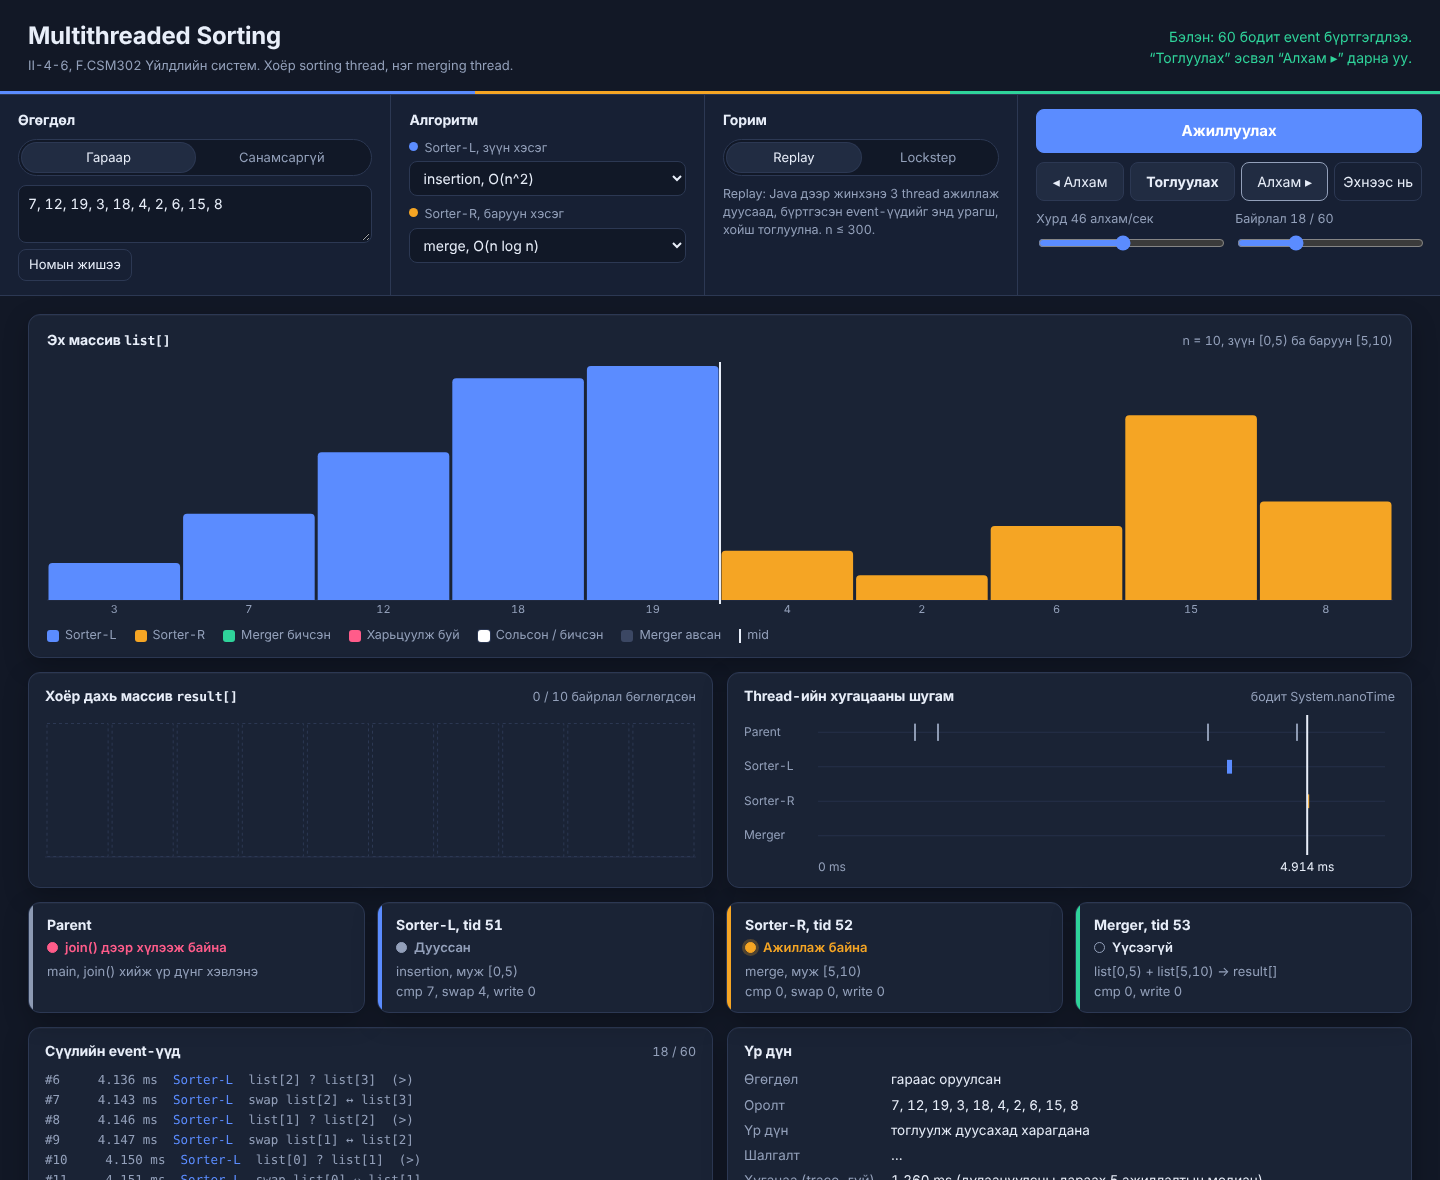
\includegraphics[width=\linewidth]{02-replay-sorting.png}
\caption{Sorter-L хэсгээ эрэмбэлж дууссан, Sorter-R ажиллаж байна}
\end{subfigure}\hfill
\begin{subfigure}{0.49\linewidth}\centering
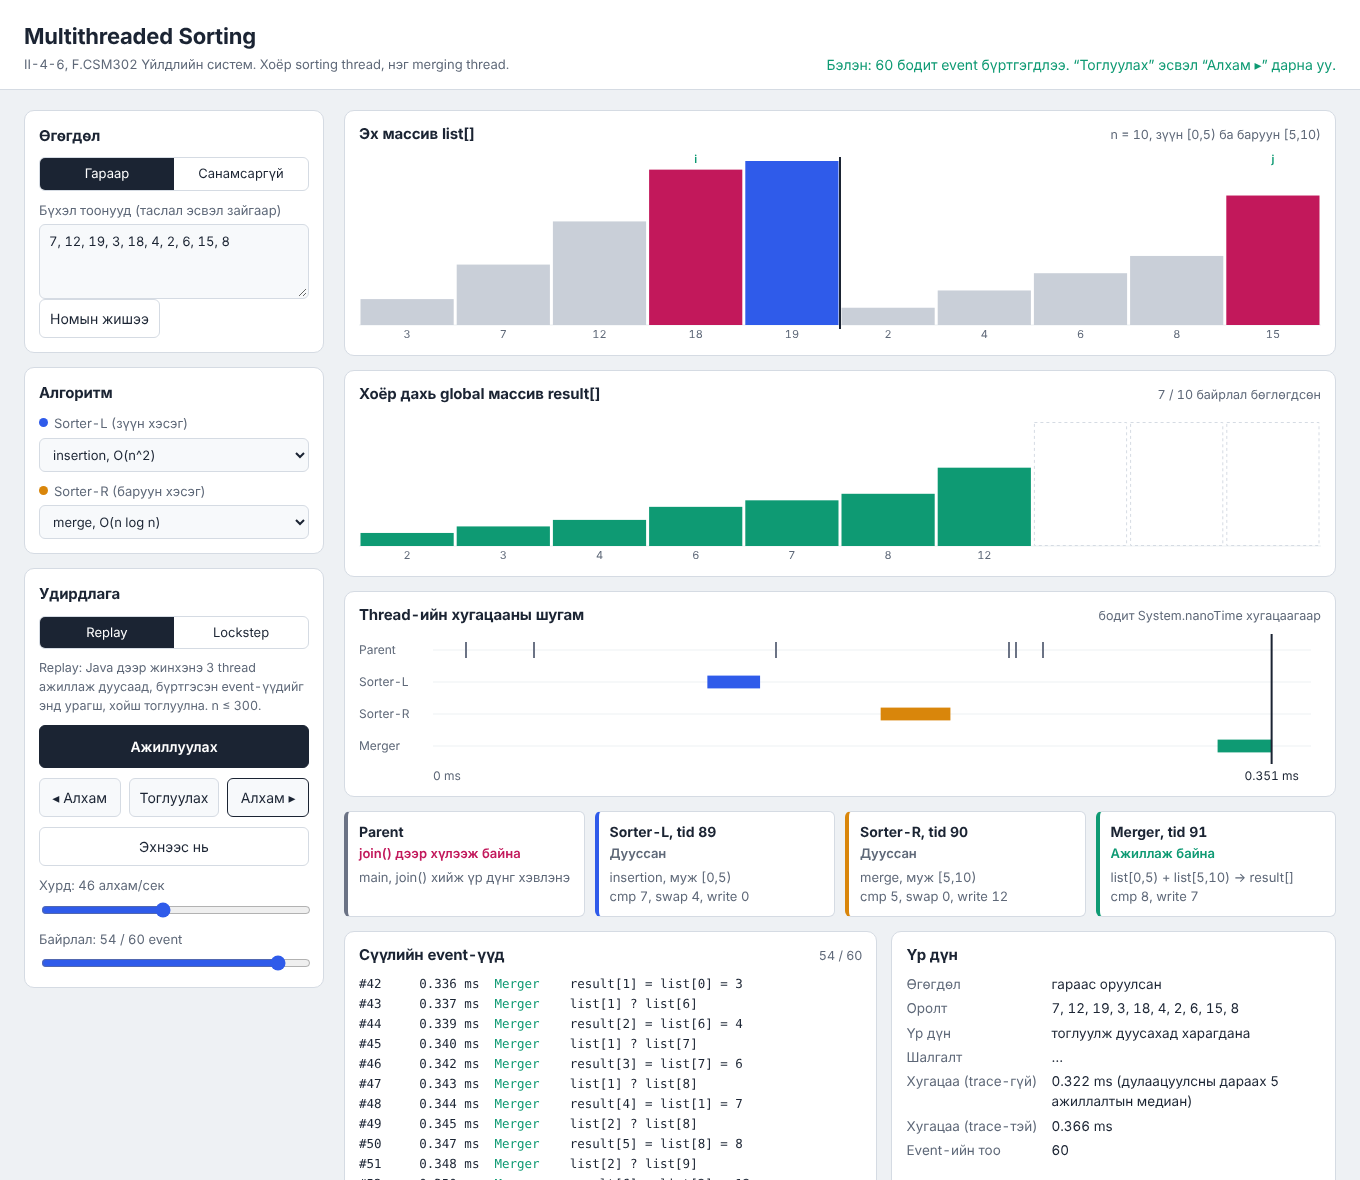
\includegraphics[width=\linewidth]{03-replay-merge.png}
\caption{Merger \code{result[]} руу нэгтгэж байна}
\end{subfigure}
\caption{Replay горим, номын жишээ}\label{fig:ui}
\end{figure}

\section{Replay ба Lockstep горим}
\textbf{Replay} горимд сервер бодит 3 thread-ийг ажиллуулж, бүх event-ийг хөтөч рүү буцаана. Хөтөч эхний $k$
event-ийг эх жагсаалт дээр хэрэглэж дурын алхамд очих тул урагш, хойш явах боломжтой. Мөн trace-гүй ажиллалтын
хугацааг тусад нь харуулна.

\textbf{Lockstep} горимд thread-үүд амьд хэвээр байж, үйлдэл бүрийн өмнө Semaphore дээр зогсоно. “Алхам” бүр
серверт нэг permit өгч, шинэ event-үүд болон thread бүрийн \code{Thread.getState()}-ийг авна (Зураг~\ref{fig:ui-lockstep}).
Бодит thread-ийг буцааж болохгүй тул энэ горимд хойш алхах боломжгүй. Хугацааны тэмдэглэгээ нь хэрэглэгчийн товч
дарах хоорондын хугацааг агуулдаг тул хурд хэмжихэд Replay горимыг ашиглана.

\begin{figure}[H]
\centering
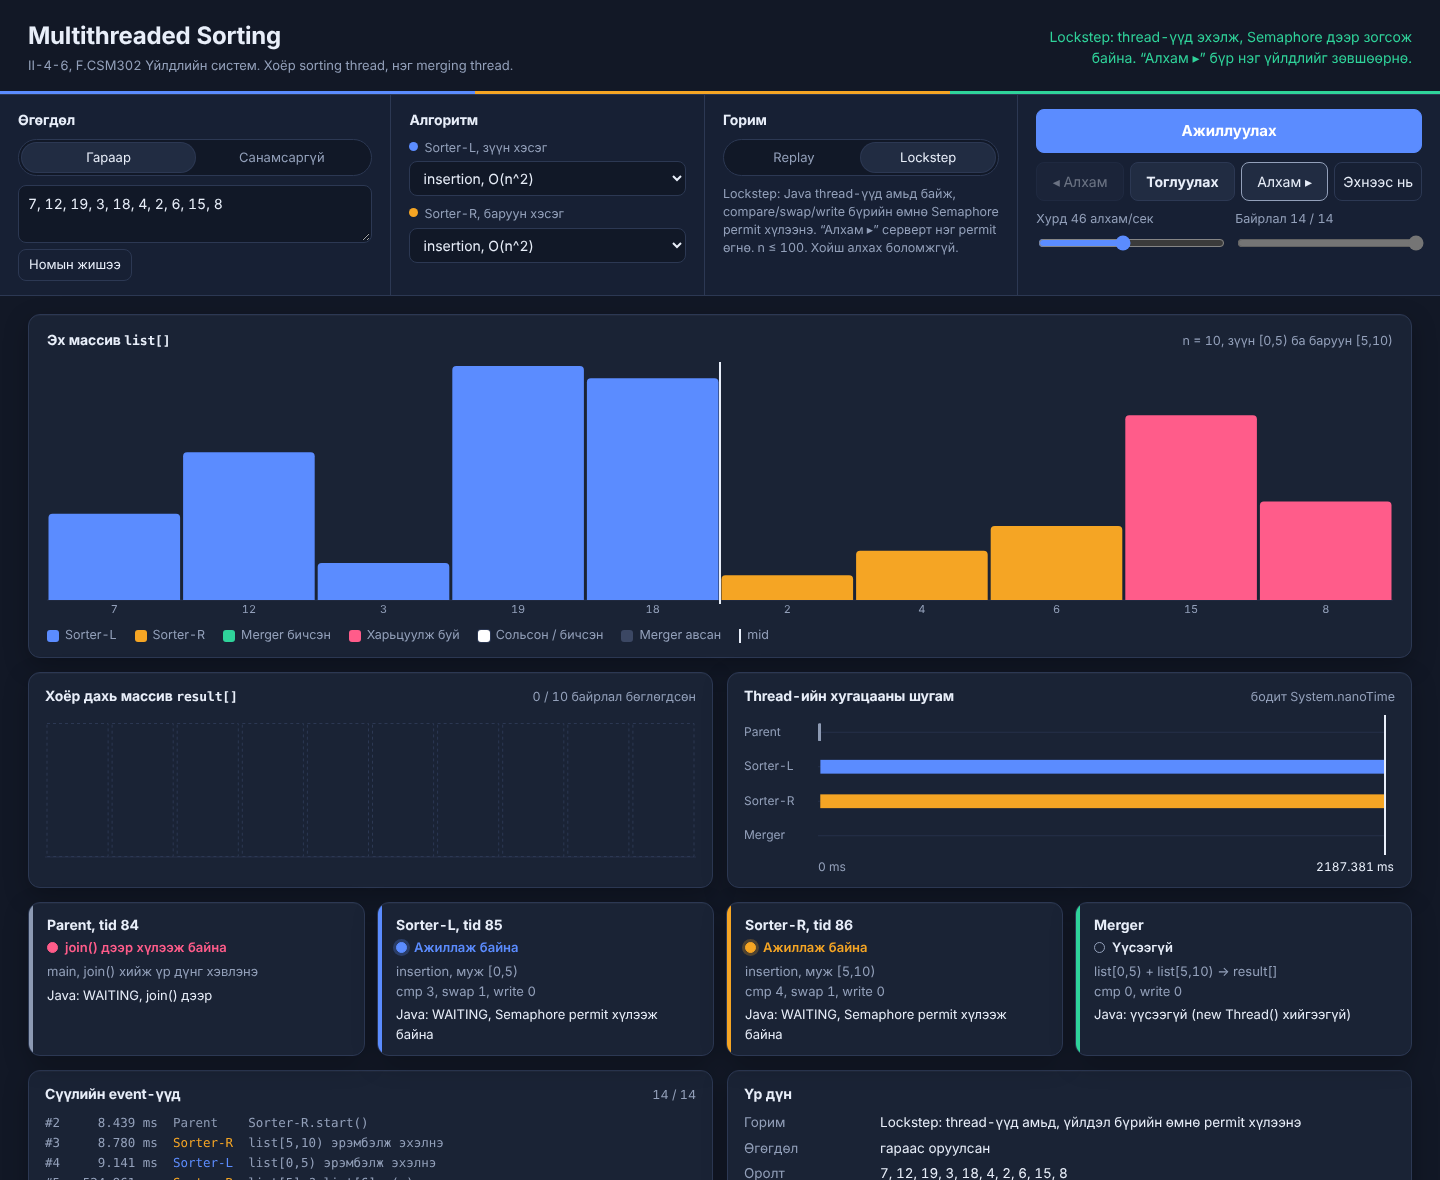
\includegraphics[width=0.72\linewidth]{06-lockstep.png}
\caption{Lockstep: хоёр sorter Semaphore дээр \code{WAITING}, parent \code{join()} дээр \code{WAITING}}\label{fig:ui-lockstep}
\end{figure}

% !TEX root = ../main.tex
\chapter{Туршилтын арга}\label{ch:method}

\section{Орчин}
Тестийг багийн гишүүний компьютер (macOS 27, Apple Silicon, 10 цөм, Eclipse Temurin 17.0.21) болон хөгжүүлэлтийн
Linux контейнер (Ubuntu 24.04, Intel Xeon, 2 цөм, OpenJDK 21) дээр ажиллуулав. Хугацааны хэмжилтийг контейнер дээр хийсэн.

\section{Автомат тест}
Тестийг JUnit-гүй, \code{tests/TestRunner.java} файлд бичсэн бөгөөд \code{./test.sh} ажиллуулна. Тест бүрд
урьдчилан бичсэн хүлээгдсэн үр дүн ба програмын бодит үр дүнг харьцуулж, бүх эрэмбэлэлтийг \code{Arrays.sort}-той
тулгана. Үр дүнгийн хүснэгт \code{tests/results/test-results.md}-д бичигдэнэ.

\begin{table}[H]
\centering\small
\caption{Автомат тестийн ангилал}\label{tab:tests}
\begin{tabularx}{\linewidth}{@{}lrY@{}}
\toprule
Ангилал & Тоо & Шалгах зүйл \\
\midrule
Номын жишээ & 26 & 25 алгоритмын хослол, mid = 5, хоёр хэсэг \\
Захын тохиолдол & 17 & $n = 1, 2, 3$, бүгд ижил, сөрөг, INT\_MIN/MAX, эрэмбэтэй, урвуу, $\lceil n/2\rceil$ / $\lfloor n/2\rfloor$ \\
Буруу оролт & 18 & Хоосон, тоо биш, бутархай, int-ээс гадуур, хязгаарууд, буруу файл \\
Давхардал ба хэлбэр & 6 & 4 хэлбэр × 25 хослол, 2000 санамсаргүй ажиллалт \\
Том өгөгдөл & 4 & $n = 10^6$ (merge, quick), $n = 20\,000$ (O($n^2$)) \\
Thread & 5 & 3 өөр thread, параметр, \code{TERMINATED}, дараалал, муж зөрчөөгүй \\
Event trace & 7 & Trace-ээс сэргээсэн \code{result[]} = бодит, JSON формат \\
Lockstep & 5 & \code{WAITING}, 1 permit = 1 үйлдэл, ээлжлэх, цуцлах \\
Командын мөр & 12 & Тусдаа JVM дээр гаралт ба exit code \\
\bottomrule
\end{tabularx}
\end{table}

Тест нь зөвхөн үр дүнг биш, номын дотоод нөхцлийг ч шалгадаг. Trace-ийн бүх event-ээр Sorter-L нь
\code{[0, mid)}-ээс, Sorter-R нь \code{[mid, n)}-ээс гадуур хандаагүйг баталсан. Мөн merger хоёр sorter дууссаны дараа
эхэлснийг 100 удаа шалгасан. Lockstep-ийн тестийг 30 удаа дараалан болон нэг цөм дээр (\code{taskset -c 0}) ажиллуулсан.
Web UI-г Playwright (Chromium)-оор автоматаар шалгаж, JavaScript алдаа 0 байгааг баталсан.

\section{Хугацааны хэмжилтийн арга}
\code{tests/Benchmark.java} (\code{./bench.sh}) нь гурван хувилбарыг харьцуулна: \emph{1 thread} (нэг thread бүх массивыг
эрэмбэлнэ), \emph{1 thread, хувааж} (номын бүтэцтэй ижил ажлыг нэг thread дараалан хийнэ) ба \emph{3 thread} (номын
бүтэц). Нийт хурдсалт $= T_{1}/T_{3}$, зэрэгцээний хурдсалт $= T_{1,\text{хувааж}}/T_{3}$. Хоёр дахь нь хуваалтын
нөлөөг зэрэгцээний нөлөөнөөс салгана. Оролт санамсаргүй \code{int}, trace унтраалттай. JIT-ийн нөлөөг багасгахын тулд
3 тусдаа JVM ажиллуулж, тус бүрд 3 удаа дулаацуулсны дараа 9 удаа хэмжиж, медианы медианыг авсан.

% !TEX root = ../main.tex
\chapter{Үр дүн}\label{ch:results}\label{ch:perf}

\section{Тестийн үр дүн}
100 автомат тест хоёр орчинд хоёуланд нь амжилттай (100/100) болсон. Lockstep-ийн тестийг 30 удаа давтаж,
нэг цөм дээр ажиллуулахад ч алдаа гараагүй. Тест бүрийн оролт, хүлээгдсэн ба бодит утгыг
\code{tests/results/test-results.md}-д өгөв.

\begin{figure}[H]
\centering
\IfFileExists{images/test-run-mac.png}{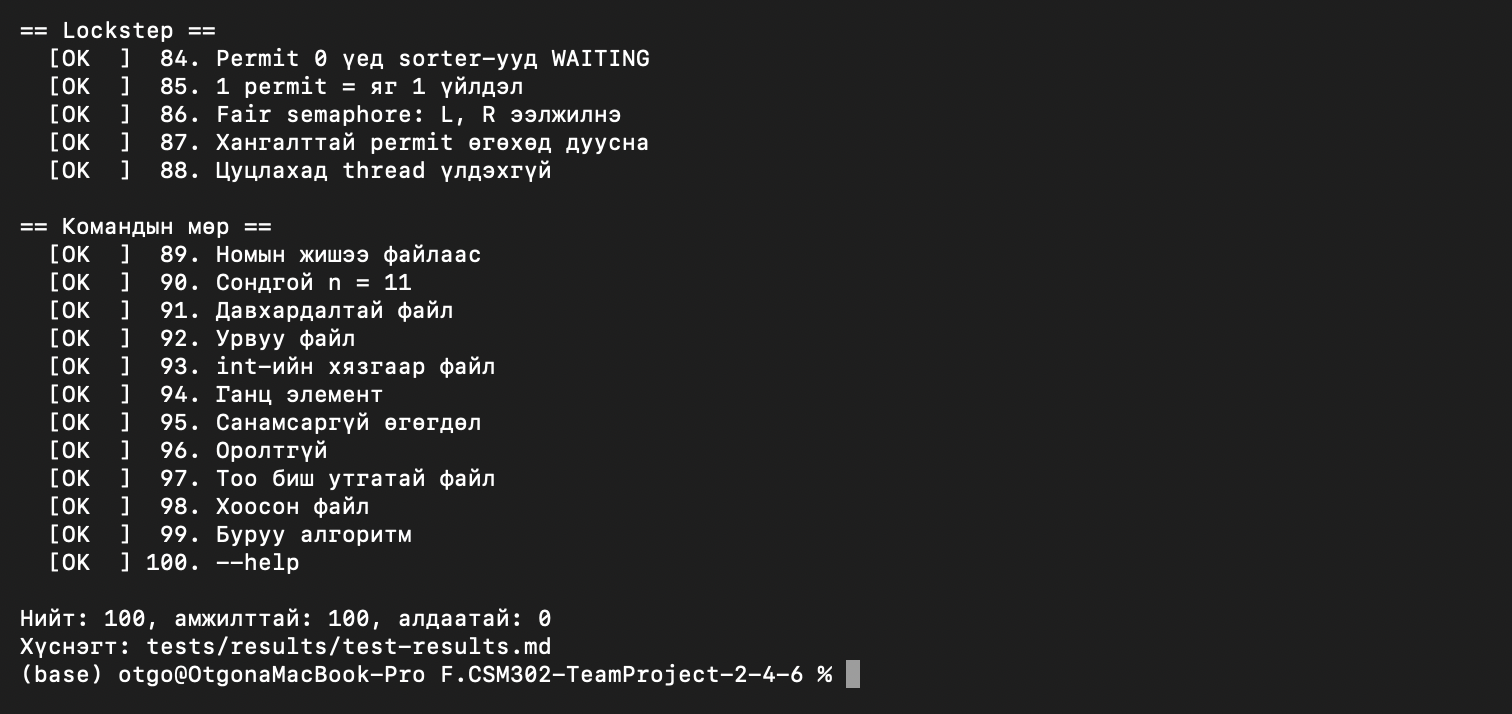
\includegraphics[width=0.7\linewidth]{images/test-run-mac.png}}{%
\fbox{\parbox[c][3cm][c]{0.7\linewidth}{\centering\color{cparent}Энд зураг оруулна: \texttt{report/images/test-run-mac.png}}}}
\caption{\code{./test.sh}-ийн гаралт}\label{fig:testrun}
\end{figure}

\section{Хугацааны хэмжилтийн үр дүн}
Хүснэгт~\ref{tab:bench}-т $n$-ийн хамгийн том утгууд дээрх үр дүнг, Зураг~\ref{fig:bench-speedup}-т зэрэгцээний
хурдсалтыг $n$-ээс хамааруулан харуулав. Бүрэн үр дүн \code{tests/results/benchmark.md}-д бий.

\begin{table}[H]
\centering
\caption{Хугацаа (ms, медиан). Хаалтанд 3 thread-ийн JVM хоорондын муж}\label{tab:bench}
\resizebox{\linewidth}{!}{%
\begin{tabular}{@{}lrrrrrrr@{}}
\toprule
Алгоритм & $n$ & 1 thread & 1 thr., хувааж & 3 thread & Нэгтгэх үе & Нийт & Зэрэгц. \\
\midrule
insertion & 20 000 & 180.1 & 90.6 & 50.6 (48.3--54.3) & 0.7 & 3.56 & 1.79 \\
bubble & 20 000 & 466.1 & 198.5 & 73.9 (67.0--145.4) & 0.5 & 6.30 & 2.68 \\
selection & 20 000 & 152.5 & 74.2 & 62.2 (45.9--65.1) & 0.7 & 2.45 & 1.19 \\
merge & 100 000 & 13.9 & 13.7 & 10.4 (9.2--10.4) & 1.1 & 1.34 & 1.32 \\
merge & 1 000 000 & 168.3 & 165.3 & 95.0 (92.8--101.5) & 7.9 & 1.77 & 1.74 \\
quick & 100 000 & 13.7 & 13.6 & 8.2 (8.0--9.4) & 1.0 & 1.66 & 1.66 \\
quick & 1 000 000 & 159.6 & 159.8 & 92.5 (92.3--99.8) & 7.4 & 1.73 & 1.73 \\
\bottomrule
\end{tabular}}
\end{table}

\begin{figure}[H]
\centering
\begin{tikzpicture}
\begin{semilogxaxis}[width=0.8\linewidth, height=6cm, xlabel={$n$}, ylabel={зэрэгцээний хурдсалт},
  ymin=0, ymax=3, grid=major, legend style={at={(0.5,-0.22)}, anchor=north, font=\scriptsize}, legend columns=5,
  tick label style={font=\scriptsize}]
  \addplot+[cleft, mark=square*, thick, only={algo}{insertion}] table[col sep=comma, x=n, y=parallel_speedup] {\benchcsv};
  \addplot+[cright, mark=triangle*, thick, only={algo}{bubble}] table[col sep=comma, x=n, y=parallel_speedup] {\benchcsv};
  \addplot+[ccmp, mark=diamond*, thick, only={algo}{selection}] table[col sep=comma, x=n, y=parallel_speedup] {\benchcsv};
  \addplot+[cmerge, mark=*, thick, only={algo}{merge}] table[col sep=comma, x=n, y=parallel_speedup] {\benchcsv};
  \addplot+[cink, mark=pentagon*, thick, only={algo}{quick}] table[col sep=comma, x=n, y=parallel_speedup] {\benchcsv};
  \addplot[cparent, dashed, domain=800:1.2e6, samples=2] {1};
  \addplot[cparent, dotted, thick, domain=800:1.2e6, samples=2] {2};
  \legend{insertion, bubble, selection, merge, quick}
\end{semilogxaxis}
\end{tikzpicture}
\caption{Зэрэгцээний хурдсалт ($T_{1\,\text{thread, хувааж}} / T_{3\,\text{thread}}$). Тасархай шугам 1 (ашиггүй), цэгэн шугам 2 (2 цөмийн онолын дээд хязгаар)}
\label{fig:bench-speedup}
\end{figure}

Жижиг $n$ дээр 3 thread-тэй хувилбар удаан байсан: $n = 100$ үед 1 thread 0.006 ms, 3 thread 0.33 ms (insertion),
$n = 1000$ үед merge sort 0.10 ба 0.50 ms. Энэ зөрүү бараг бүхэлдээ thread үүсгэх, \code{join()} хийх зардал юм.
Event trace нь $n = 1000$ үед merge sort-ыг 2.2 дахин (18\,694 event), insertion sort-ыг 43.7 дахин (245\,187 event)
удаашруулсан. Тиймээс хурдыг trace-гүй хэмжсэн.

\section{Илэрсэн ба зассан алдаа}\label{sec:bugs}
Хөгжүүлэлт, тестийн явцад дараах алдааг илрүүлж зассан:
(1) O($n^2$) алгоритмын trace-ийн хязгаар хэт их байсан тул 2 сая event-ийн дээд хязгаарт хүрч, 156 MB файл үүсч байсныг
$n \le 1000$ болгов. (2) Хоосон талбарыг \code{Integer.MIN\_VALUE}-ээр тэмдэглэдэг тул $-2^{31}$ утга trace-ээс алга болж
байсныг \code{long} талбар болгож засав. (3) UI-ийн байрлалын гулсуурыг чирэхэд хуучин байрлал руу буцдаг байсныг засав.
(4) Lockstep-ээс Replay руу шилжихэд хуучин session серверт үлддэг байсныг цуцалдаг болгов. (5) Fair semaphore үргэлж L-ээс
эхэлнэ гэж үзсэн тест давтан ажиллуулахад унасан тул “ээлжилсэн” эсэхийг шалгадаг болгов.

% !TEX root = ../main.tex
\chapter{Хэлэлцүүлэг}\label{ch:disc}

\section{Үр дүнгийн тайлбар}
Merge ба quick sort-д “1 thread” ба “1 thread, хувааж” хугацаа бараг тэнцүү. Учир нь хоёр хэсэгт хуваах нь
ажлыг багасгадаггүй: $2\cdot\frac{n}{2}\log\frac{n}{2} \approx n\log n$. Иймээс 1.73--1.77 хурдсалт бүхэлдээ
зэрэгцээнээс ирж байна. $n = 10^6$ үед merge sort-ын нэгтгэх үе 7.9 ms бөгөөд энэ нь ажлын
$S \approx 7.9/165.3 \approx 0.048$ хувь. Амдалын хуулиар~(\ref{eq:amdahl}) $N = 2$ үед дээд хязгаар
$1/(0.048 + 0.952/2) \approx 1.91$. Хэмжсэн 1.74 нь үүнээс бага бөгөөд зөрүүг thread үүсгэх зардал болон хоёр
цөмийн санах ойн шугамыг хуваалцдагтай холбож тайлбарлаж байна.

O($n^2$) алгоритмд хуваалт өөрөө ажлыг 2 дахин багасгадаг: $2\cdot(n/2)^2 = n^2/2$ (insertion 180 → 91 ms). Үүн
дээр зэрэгцээний ашиг нэмэгдэж, онолын нийт хурдсалт 4 болно. Insertion sort-ын 3.56 үүнд ойрхон байна. Иймээс
“O($n^2$) алгоритмд 2 thread 3.5 дахин хурдан” гэж дүгнэх нь төөрөгдөл бөгөөд ашгийн тал орчим нь алгоритмын
шинж чанараас ирж байгаа юм. Олон урсгалт хувилбар merge/quick-д $n \approx 10^5$-аас, O($n^2$)-д $n \approx 5000$-аас
эхэлж ашигтай болсон. Үүнээс бага $n$-д thread-ийн зардал давамгайлна. Жишээ нь номын жишээн дээр Sorter-L нь
Sorter-R эхлэхээс өмнө дуусчихдаг. Энэ нь алдаа биш, thread үүсгэх нь 5 элемент эрэмбэлэхээс удаан байдагтай холбоотой.

Lockstep горимд хоёр sorter L, R, L, R гэж хатуу ээлжилсэн. Эхэндээ үүнийг OS-ийн scheduler шийддэг гэж үзсэн боловч
шалтгаан нь fair semaphore-ийн FIFO дараалал байв. Харин эхний permit-ийг аль sorter авахыг scheduler шийддэг.

\section{Хязгаарлалт}\label{sec:limitations}
Хэмжилтийг 2 цөмтэй виртуал машин дээр хийсэн тул JIT ба GC-ийн туслах thread-үүд sorter-уудтай цөмийн төлөө
өрсөлддөг. Bubble sort-ын 3 thread-ийн хугацаа JVM-ээс хамаарч 67--145 ms хооронд хэлбэлзсэн бөгөөд түүний
зэрэгцээний хурдсалт 2.68 нь 2 цөмийн физик хязгаараас давсан. Иймд энэ утгыг JIT-ийн нөлөө гэж үзэж итгэл муутай
гэж тооцсон. 1 ms-ээс бага хугацаа шуугиантай. Windows-ийн \code{.bat} скриптийг бодит Windows машин дээр туршаагүй.

\section{Сайжруулах боломж}
$k$ sorting thread бүхий мод хэлбэрийн нэгтгэл нь олон цөмийг бүрэн ашиглана. Нэгтгэх үеийг хоёр thread-д хуваавал
(нэг нь эхнээс, нөгөө нь төгсгөлөөс) Амдалын $S$ багасна. Thread pool болон босго утга (жижиг $n$-д дан thread)
ашиглавал жижиг өгөгдлийн зардал буурна. \code{Arrays.parallelSort} ч мөн ийм босго ашигладаг~\cite{javadoc-arrays}.

\section{GitHub ба AI ашигласан тухай}
\code{22dbddf} ба \code{a8916d6} commit-ууд ижил мессежтэй. Учир нь web UI-г шалгалт дуусахаас өмнө commit хийсэн
тул засвар нь дараагийн commit-д орсон. Хуваалцсан түүхийг \code{force push}-оор өөрчлөхгүйн тулд хэвээр үлдээв.

Төслийн код, тест, гарын авлага, тайлангийн нооргийг бэлтгэхэд Claude хиймэл оюун ухаан ашигласан.
Бүх \code{git} үйлдлийг багийн гишүүд өөрсдөө хийсэн. Гишүүд AI-ийн үүсгэсэн материалыг уншиж, засварлаж, програмыг
өөрсдийн компьютер дээр ажиллуулж шалгасан. Тайлан дахь тоо бүр програмыг бодитоор ажиллуулж гарсан утга юм.

% !TEX root = ../main.tex
\chapter{Дүгнэлт}\label{ch:concl}

“Multithreaded Sorting Application” төслийг Java 17 дээр бүрэн хэрэгжүүлэв. Програм жагсаалтыг хоёр хуваан хоёр
sorting thread-ээр параметрээр өгсөн мужийг эрэмбэлж, merging thread-ээр хоёр дахь global массив руу нэгтгэнэ. Parent
thread бүх thread-ийг \code{join()} хийсний дараа үр дүнг хэвлэнэ. Үүн дээр таван алгоритм, оролтын бүрэн шалгалт,
JSON event trace, бодит thread-тэй холбогдсон Sorting animation (Replay ба Lockstep горим) хийж, 100 автомат тестээр
шалгасан.

Ажлын гол сургамж нь гурав. Нэгдүгээрт, \code{start()}/\code{join()} нь өөрөө синхрончлол бөгөөд давхцахгүй муж ба
join-ийн дарааллын ачаар lock огт хэрэггүй. Хоёрдугаарт, зэрэгцээ нь үнэгүй биш: жижиг $n$-д thread-ийн зардал
давамгайлж, их $n$-д ч нэгтгэх дан үеэс болж хурдсалт 2-т хүрэхгүй (Амдалын хууль). Гуравдугаарт, хурдсалтыг зөв
тайлбарлахын тулд “1 thread, хувааж” гэх мэт тохирох суурь хэмжилт болон олон JVM-ийн медиан шаардлагатай.
Цаашид олон thread бүхий мод хэлбэрийн нэгтгэл, зэрэгцээ merge ашиглаж олон цөмийг илүү бүрэн ашиглах боломжтой.


% !TEX root = ../main.tex
% ---------------------------------------------------------------- ном зүй
\begin{thebibliography}{99}
\addcontentsline{toc}{chapter}{Ашигласан материал}

\bibitem{osc10}
A. Silberschatz, P. B. Galvin, G. Gagne.
\emph{Operating System Concepts}, 10th ed. Hoboken, NJ: Wiley, 2018.
Chapter 4 “Threads \& Concurrency”, Chapter 6 “Synchronization Tools”.

\bibitem{amdahl67}
G. M. Amdahl. “Validity of the single processor approach to achieving large scale computing capabilities.”
In \emph{Proc. AFIPS Spring Joint Computer Conference}, pp. 483--485, 1967.

\bibitem{jls17}
J. Gosling, B. Joy, G. Steele, G. Bracha, A. Buckley, D. Smith, G. Bierman.
\emph{The Java Language Specification, Java SE 17 Edition}, Chapter 17 “Threads and Locks”. Oracle, 2021.
\url{https://docs.oracle.com/javase/specs/jls/se17/html/jls-17.html}

\bibitem{javadoc-thread}
Oracle. \emph{Java SE 17 API: \texttt{java.lang.Thread}, \texttt{Thread.State}}.
\url{https://docs.oracle.com/en/java/javase/17/docs/api/java.base/java/lang/Thread.html}

\bibitem{javadoc-semaphore}
Oracle. \emph{Java SE 17 API: \texttt{java.util.concurrent.Semaphore}}.
\url{https://docs.oracle.com/en/java/javase/17/docs/api/java.base/java/util/concurrent/Semaphore.html}

\bibitem{javadoc-arrays}
Oracle. \emph{Java SE 17 API: \texttt{java.util.Arrays.parallelSort}}.
\url{https://docs.oracle.com/en/java/javase/17/docs/api/java.base/java/util/Arrays.html}

\bibitem{goetz}
B. Goetz, T. Peierls, J. Bloch, J. Bowbeer, D. Holmes, D. Lea.
\emph{Java Concurrency in Practice}. Addison-Wesley, 2006.

\bibitem{clrs}
T. H. Cormen, C. E. Leiserson, R. L. Rivest, C. Stein.
\emph{Introduction to Algorithms}, 4th ed. MIT Press, 2022.

\bibitem{hoare62}
C. A. R. Hoare. “Quicksort.” \emph{The Computer Journal}, 5(1):10--16, 1962.

\bibitem{repo}
Багийн GitHub repository. \url{https://github.com/Munkhgerelt/F.CSM302-TeamProject-2-4-6}

\end{thebibliography}



\end{document}
